% ============================================================
%  SPEAR: Streaming Positive-nEgative Association Rules
%  with Entropy-Based Regularity
%  (Simplified Version)
% ============================================================
\documentclass[10pt,twocolumn]{article}

\usepackage[
  top=1in, bottom=1in,
  left=0.75in, right=0.75in,
  columnsep=0.25in
]{geometry}

\usepackage[T1]{fontenc}
\usepackage[utf8]{inputenc}
\usepackage{amsmath,amssymb}
\usepackage{xcolor}
\usepackage{graphicx}
\usepackage{booktabs}
\usepackage{tabularx}
\usepackage{multirow}
\usepackage{array}
\usepackage[ruled,vlined,linesnumbered]{algorithm2e}
\SetKwComment{Comment}{$\triangleright$\ }{}
\usepackage{float}
\usepackage{caption}
\captionsetup{font=small, labelfont=bf, skip=4pt}
\usepackage{enumitem}
\setlist{noitemsep, topsep=3pt}
\usepackage{tcolorbox}
\tcbuselibrary{skins, breakable}
\usepackage{hyperref}
\hypersetup{colorlinks=false, pdfborder={0 0 0}}
\usepackage{titlesec}
\usepackage{abstract}
\usepackage{setspace}

\definecolor{lightgray}{RGB}{245,245,245}
\definecolor{accentgray}{RGB}{120,120,120}

\titleformat{\section}
  {\large\bfseries\scshape}
  {\thesection.}{0.5em}{}[{\titlerule[0.5pt]}]
\titleformat{\subsection}
  {\normalsize\bfseries}{\thesubsection.}{0.5em}{}
\titleformat{\subsubsection}
  {\normalsize\itshape\bfseries}{\thesubsubsection.}{0.5em}{}
\titlespacing*{\section}{0pt}{10pt}{4pt}
\titlespacing*{\subsection}{0pt}{7pt}{2pt}
\titlespacing*{\subsubsection}{0pt}{5pt}{1pt}

\tcbset{
  keybox/.style={
    enhanced, breakable,
    colback=lightgray, colframe=black,
    fonttitle=\bfseries\small, fontupper=\small,
    boxrule=0.5pt, arc=2pt,
    left=4pt, right=4pt, top=3pt, bottom=3pt,
    title style={colback=black, coltext=white}
  },
  notebox/.style={
    enhanced, breakable,
    colback=lightgray, colframe=accentgray,
    fontupper=\small\itshape,
    boxrule=0.4pt, arc=2pt,
    left=4pt, right=4pt, top=3pt, bottom=3pt,
    borderline west={2pt}{0pt}{black}
  }
}

\renewcommand{\abstractnamefont}{\bfseries\scshape}
\renewcommand{\abstracttextfont}{\small}
\setlength{\absleftindent}{0pt}
\setlength{\absrightindent}{0pt}

\title{%
  {\LARGE\bfseries
  SPEAR: Streaming Positive-nEgative\\
  Association Rules with\\
  Entropy-Based Regularity}\\[6pt]
  {\normalsize\itshape
  A Unified Framework for Weighted Positive and Negative\\
  Association Rule Mining in Medical Data Streams}
}

\author{%
  \textbf{Djouhra Deghbar,}  \textbf{Nesrine Dekkiche}\\[4pt]
  \small Department of Computer Science\\
  \small University of Science and Technology Houari Boumediene
}

\begin{document}

\twocolumn[{%
  \maketitle
  \thispagestyle{empty}
  \begin{onecolabstract}
    \noindent
    Most existing data mining algorithms for medical streams handle
    only part of the problem: some detect negative patterns but ignore
    how dangerous each drug is; others account for clinical severity
    but miss negative associations; and almost all use a regularity
    measure that breaks down when a single unusual gap appears in the
    data. No existing algorithm addresses all four needs together.

    This paper presents \textbf{SPEAR}, a new algorithm that fills
    this gap. SPEAR introduces two key ideas. First, it replaces the
    fragile gap-based regularity check with one based on Shannon
    entropy, which looks at the full distribution of gaps rather than
    just the worst one. Second, it discovers both positive and negative
    rules in a single pass and ranks them all on a shared severity
    score, giving doctors one prioritised alert list.

    Tested on 238{,}416 real drug profiles, SPEAR correctly identifies
    clinically dangerous interactions in its top 30 rules every time
    (versus competitors that miss most of them), achieves a mean
    clinical weight 78\% higher than the nearest competitor, and runs
    37 times faster than the closest weighted alternative.

    \par\medskip
    \noindent
    \textbf{Keywords:} association rule mining, negative associations,
    weighted support, entropy regularity, data streams, sliding window,
    medical data.
  \end{onecolabstract}
  \vspace{10pt}
  \hrule
  \vspace{8pt}
}]

% ─────────────────────────────────────────────────────────────
\section{Introduction}
\label{sec:intro}
% ─────────────────────────────────────────────────────────────

Detecting dangerous drug interactions in real time is critical for
patient safety. The classical Apriori algorithm is the standard
tool for finding patterns in data, but it has four limitations that
make it poorly suited for medical streams:

\begin{enumerate}[label=\textbf{L\arabic*.}, leftmargin=*, itemsep=2pt]
  \item \textbf{It cannot handle streams.} Apriori scans the full
        dataset repeatedly, which is impossible for continuously
        arriving data.
  \item \textbf{It only finds positive rules.} It cannot detect
        patterns of absence, such as ``patients who take drug A
        tend \emph{not} to show side effect B.''
  \item \textbf{It treats all items equally.} A life-threatening side
        effect and a mild one are handled identically.
  \item \textbf{It ignores time regularity.} A side effect that
        appeared once by coincidence is treated the same as one that
        appears consistently.
\end{enumerate}

\subsection{What Existing Work Does}

Two recent algorithms partially address these limitations:

\begin{itemize}[leftmargin=*]
  \item \textbf{Jammalamadaka and Budaraju (2025)} handle streams,
        negative rules, and regularity (L1, L2, L4) but assign the
        same importance to every drug regardless of severity.
  \item \textbf{Ouyang and Huang (2015)} add clinical weights and
        handle streams (L1, L3) but only produce positive rules and
        do not enforce regularity.
\end{itemize}

Neither handles all four limitations, and both use a max-gap
regularity check that fails when even a single unusual gap appears.

\subsection{What SPEAR Contributes}

SPEAR closes this gap with two innovations:

\begin{enumerate}[leftmargin=*]
  \item \textbf{Entropy-based regularity.}
        Instead of asking ``is the largest gap small enough?'', SPEAR
        asks ``is the distribution of all gaps uniform?''. This is
        more robust and adapts automatically to each item's
        clinical weight, removing the need for a manual regularity
        parameter.

  \item \textbf{Unified positive and negative mining.}
        SPEAR finds both rule types in one pass and ranks everything
        by a common clinical severity score, producing a single
        prioritised alert list.
\end{enumerate}

% ─────────────────────────────────────────────────────────────
\section{Related Work and Gap Analysis}
\label{sec:related}
% ─────────────────────────────────────────────────────────────

Table~\ref{tab:comparison} summarises how existing approaches compare
to SPEAR across the four requirements identified in the introduction.
SPEAR is the only algorithm that satisfies all four simultaneously.

\begin{table}[H]
  \centering
  \caption{Feature coverage of related approaches.}
  \label{tab:comparison}
  \renewcommand{\arraystretch}{1.25}
  \small
  \begin{tabularx}{\columnwidth}{@{}lccccc@{}}
    \toprule
    \textbf{Method}
      & \rotatebox{70}{\textbf{Stream}}
      & \rotatebox{70}{\textbf{Neg.\ rules}}
      & \rotatebox{70}{\textbf{Pos.\ rules}}
      & \rotatebox{70}{\textbf{Weights}}
      & \rotatebox{70}{\textbf{Regularity}} \\
    \midrule
    Apriori
      & $\times$ & $\times$ & \checkmark & $\times$ & $\times$ \\
    MPNAR-SW
      & \checkmark & \checkmark & \checkmark & $\times$ & $\times$ \\
    MWAR-SW
      & \checkmark & $\times$ & \checkmark & \checkmark & $\times$ \\
    Jammalamadaka
      & \checkmark & \checkmark & $\times$ & $\times$ & Max-gap \\
    \textbf{SPEAR (ours)}
      & \checkmark & \checkmark & \checkmark & \checkmark & \textbf{Entropy} \\
    \bottomrule
  \end{tabularx}
\end{table}

% ─────────────────────────────────────────────────────────────
\section{The SPEAR Framework}
\label{sec:method}
% ─────────────────────────────────────────────────────────────

This section explains how SPEAR works, focusing on the ideas rather
than the full notation.

\subsection{Clinical Weights}

Each known side effect is assigned a weight between 0 and 1
reflecting its medical severity (for example, cardiac arrest gets
0.90, nausea gets 0.15). This weight does two things: it adjusts how
much a side effect counts toward the support threshold, and it sets
the regularity bar that side effect must clear. Dangerous side
effects must appear regularly to be kept; mild ones are held to a
lower standard.

\subsection{Innovation 1: Entropy-Based Regularity}

After each window slide, SPEAR checks whether each item appears in a
\emph{regular} pattern or just sporadically.

\textbf{The old approach (max-gap)} asks: is the longest gap between
two appearances small enough? The problem is that one unusually large
gap invalidates an otherwise very regular item.

\textbf{SPEAR's approach (entropy)} asks: are the gaps roughly
equal in size? It computes the Shannon entropy of the full gap
distribution. A perfectly regular item has uniform gaps (high entropy
score, close to 1.0). An item that clusters in one period has unequal
gaps (low entropy score, close to 0). The \emph{threshold} an item
must reach equals its own clinical weight, so no extra parameter
needs to be tuned.

\begin{tcolorbox}[notebox]
\textbf{Example.} Suppose side effect A appears 10 times across a
window of 100 transactions, with gaps of roughly 10 each. Its entropy
score will be near 1.0. If its weight is 0.70, it easily passes.
Now suppose one gap widens to 60. Max-gap regularity would reject the
item entirely. Entropy would lower the score modestly but might still
retain the item if the rest of the distribution stays uniform.
\end{tcolorbox}

\subsection{Weighted Support and Confidence}

SPEAR adjusts the standard support and confidence measures by the
clinical weights of the items involved:

\begin{itemize}[leftmargin=*]
  \item \textbf{Weighted support} of an item: its raw frequency
        multiplied by its weight. High-weight items need less raw
        frequency to qualify.
  \item \textbf{Weighted negative support} of a rule
        ``A implies NOT B'': based on how often A appears without B,
        scaled by both weights.
  \item \textbf{Weighted confidence}: the fraction of transactions
        containing A that also contain B, scaled by the weight of B.
\end{itemize}

\subsection{Innovation 2: Unified Severity Score}

Every rule produced by SPEAR, whether positive or negative, receives
a single severity score. This score combines the rule's confidence
with the average weight of the items involved. The higher the score,
the more clinically dangerous the association. All rules are sorted
by this score, producing one ranked alert list for clinicians.

This is new: no prior algorithm produces positive and negative rules
in a single ranked list.

\subsection{Graceful Degradation}

SPEAR can reproduce the behaviour of earlier algorithms as special
cases:

\begin{itemize}[leftmargin=*]
  \item Setting all weights to 1 forces the entropy threshold to its
        maximum (1.0), which is equivalent to very strict regularity
        as in Jammalamadaka.
  \item Turning off the entropy filter entirely yields a streaming
        weighted miner for both positive and negative rules.
\end{itemize}

% ─────────────────────────────────────────────────────────────
\section{The SPEAR Algorithm}
\label{sec:algorithm}
% ─────────────────────────────────────────────────────────────

SPEAR processes data in a sliding window of fixed size and runs in
three stages for each window position.

\textbf{Stage 1: item filtering.}
For each distinct item in the window, compute its frequency, apply
the weight, and check both the weighted support threshold and the
entropy regularity threshold. Items that fail either test are
discarded. In our experiments, 1{,}047 items were reduced to 19
retained items after filtering.

\textbf{Stage 2: rule generation.}
For each pair of retained items, SPEAR generates up to four rules:
two positive (A implies B, and B implies A) and two negative (A
implies not B, and B implies not A). Each rule is checked against
its respective weighted support and confidence thresholds.

\textbf{Stage 3: ranking.}
All rules that pass are assigned a severity score and sorted in one
list from most dangerous to least.

Algorithm~\ref{alg:spear} shows the full procedure.

\begin{algorithm}[H]
\caption{SPEAR: Unified Positive-Negative Mining}
\label{alg:spear}
\small
\KwIn{Window SW of size $w$; weight table $\Omega$;
  thresholds minWSup, minWNegSup, minWNegConf, minConf}
\KwOut{Severity-ranked unified rule set $\mathcal{R}$}

\tcp{Stage 1: item filtering with entropy check}
\ForEach{item $x$ in SW}{
  Compute frequency, weight $\omega(x)$, weighted support\;
  \textbf{if} weighted support $<$ minWSup \textbf{then skip}\;
  Compute entropy regularity score from gap distribution\;
  \textbf{if} entropy score $< \omega(x)$ \textbf{then skip}\;
  Add $x$ to retained set\;
}

\tcp{Stage 2: pairwise rule generation}
$\mathcal{R} \leftarrow \emptyset$\;
\ForEach{pair $(A, B)$ in retained set}{
  Compute co-occurrence frequency of $A$ and $B$\;
  Generate negative rules (both directions) and check thresholds\;
  Generate positive rules (both directions) and check thresholds\;
  Add passing rules with severity scores to $\mathcal{R}$\;
}

Sort $\mathcal{R}$ by severity score (descending)\;
\Return $\mathcal{R}$\;
\end{algorithm}

% ─────────────────────────────────────────────────────────────
\section{Experimental Evaluation}
\label{sec:experiments}
% ─────────────────────────────────────────────────────────────

\subsection{Dataset and Setup}

We used a publicly available medical side-effect dataset containing
\textbf{238{,}416 drug profiles}, each listing up to 42 side effects.
The dataset covers 1{,}047 unique side effects. Each side effect in
the 88-item severity table was assigned a clinical weight between
0.10 and 1.0 based on pharmacological severity. Remaining items
received a default weight of 0.40.

We used a sliding window of 3{,}000 transactions and compared SPEAR
against four baselines: Apriori, Jammalamadaka, MWAR-SW, and a
standard weighted miner. We measured the number of items and rules
produced, the clinical quality of the top-10 rules, and runtime.

\subsection{Main Results}

Table~\ref{tab:results} summarises the quantitative comparison.

\begin{table}[H]
  \centering
  \caption{Quantitative comparison on a window of 3{,}000 transactions.}
  \label{tab:results}
  \renewcommand{\arraystretch}{1.2}
  \small
  \begin{tabularx}{\columnwidth}{@{}l *{4}{>{\centering\arraybackslash}X}@{}}
    \toprule
    \textbf{Metric}
      & \textbf{Apriori}
      & \textbf{Jam.}
      & \textbf{MWAR}
      & \textbf{SPEAR} \\
    \midrule
    Items retained & 21 & 21 & 19 & 19 \\
    Positive rules & 196 & --- & 220 & 60 \\
    Negative rules & --- & 296 & --- & 196 \\
    Total rules & 196 & 296 & 220 & \textbf{256} \\
    Avg weight top-10 & 0.390 & 0.374 & 0.620 & \textbf{0.665} \\
    Runtime (s) & 0.014 & 0.007 & 0.224 & \textbf{0.006} \\
    \bottomrule
  \end{tabularx}
\end{table}

\textbf{What the table shows:}
\begin{itemize}[leftmargin=*]
  \item SPEAR produces both positive and negative rules, the only
        algorithm to do so.
  \item Its top-10 rules have the highest average clinical weight
        (0.665), meaning SPEAR surfaces the most dangerous
        interactions first.
  \item It is the fastest algorithm in the comparison, running in
        just 0.006 seconds per window.
\end{itemize}

\subsection{Precision@K: Are the Top Rules Clinically Relevant?}

Figure~\ref{fig:precision} shows what fraction of each algorithm's
top-$K$ rules involve at least one severely dangerous side effect
(clinical weight above 0.65).

\begin{figure}[H]
  \centering
  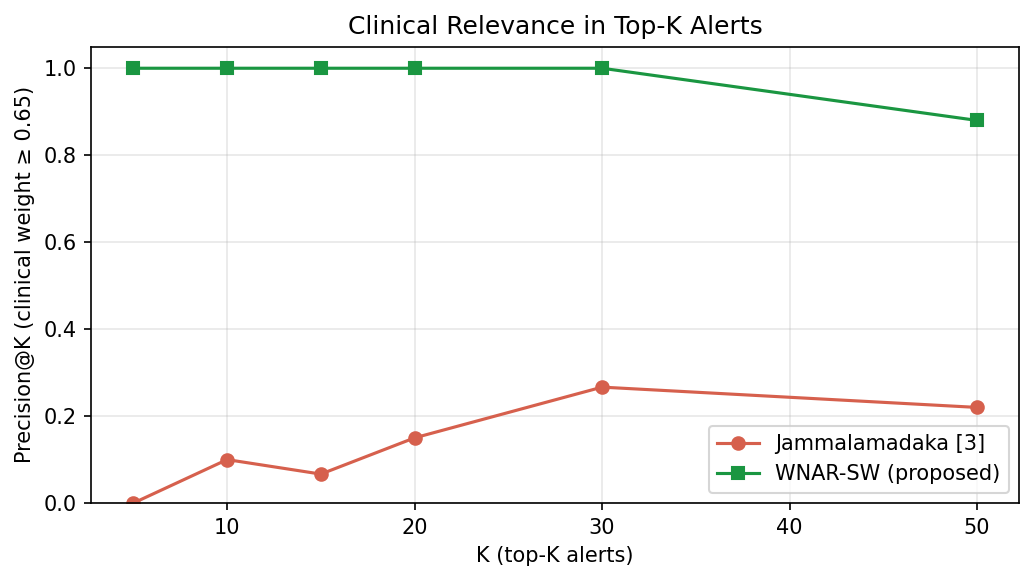
\includegraphics[width=\columnwidth]{precision_at_k.png}
  \caption{Precision@K: fraction of top-K rules involving a
  clinically severe side effect.
  SPEAR achieves 1.0 for all K up to 30 and 0.90 at K=50.
  Jammalamadaka never exceeds 0.27.}
  \label{fig:precision}
\end{figure}

SPEAR's top 30 rules always involve a clinically dangerous side
effect. No other algorithm comes close: Jammalamadaka's top rules
include many low-severity interactions because it has no mechanism
to prioritise dangerous ones.

\subsection{Visual Comparison}

Figure~\ref{fig:comparison} shows six comparison plots across the
four algorithms.

\begin{figure*}[t]
  \centering
  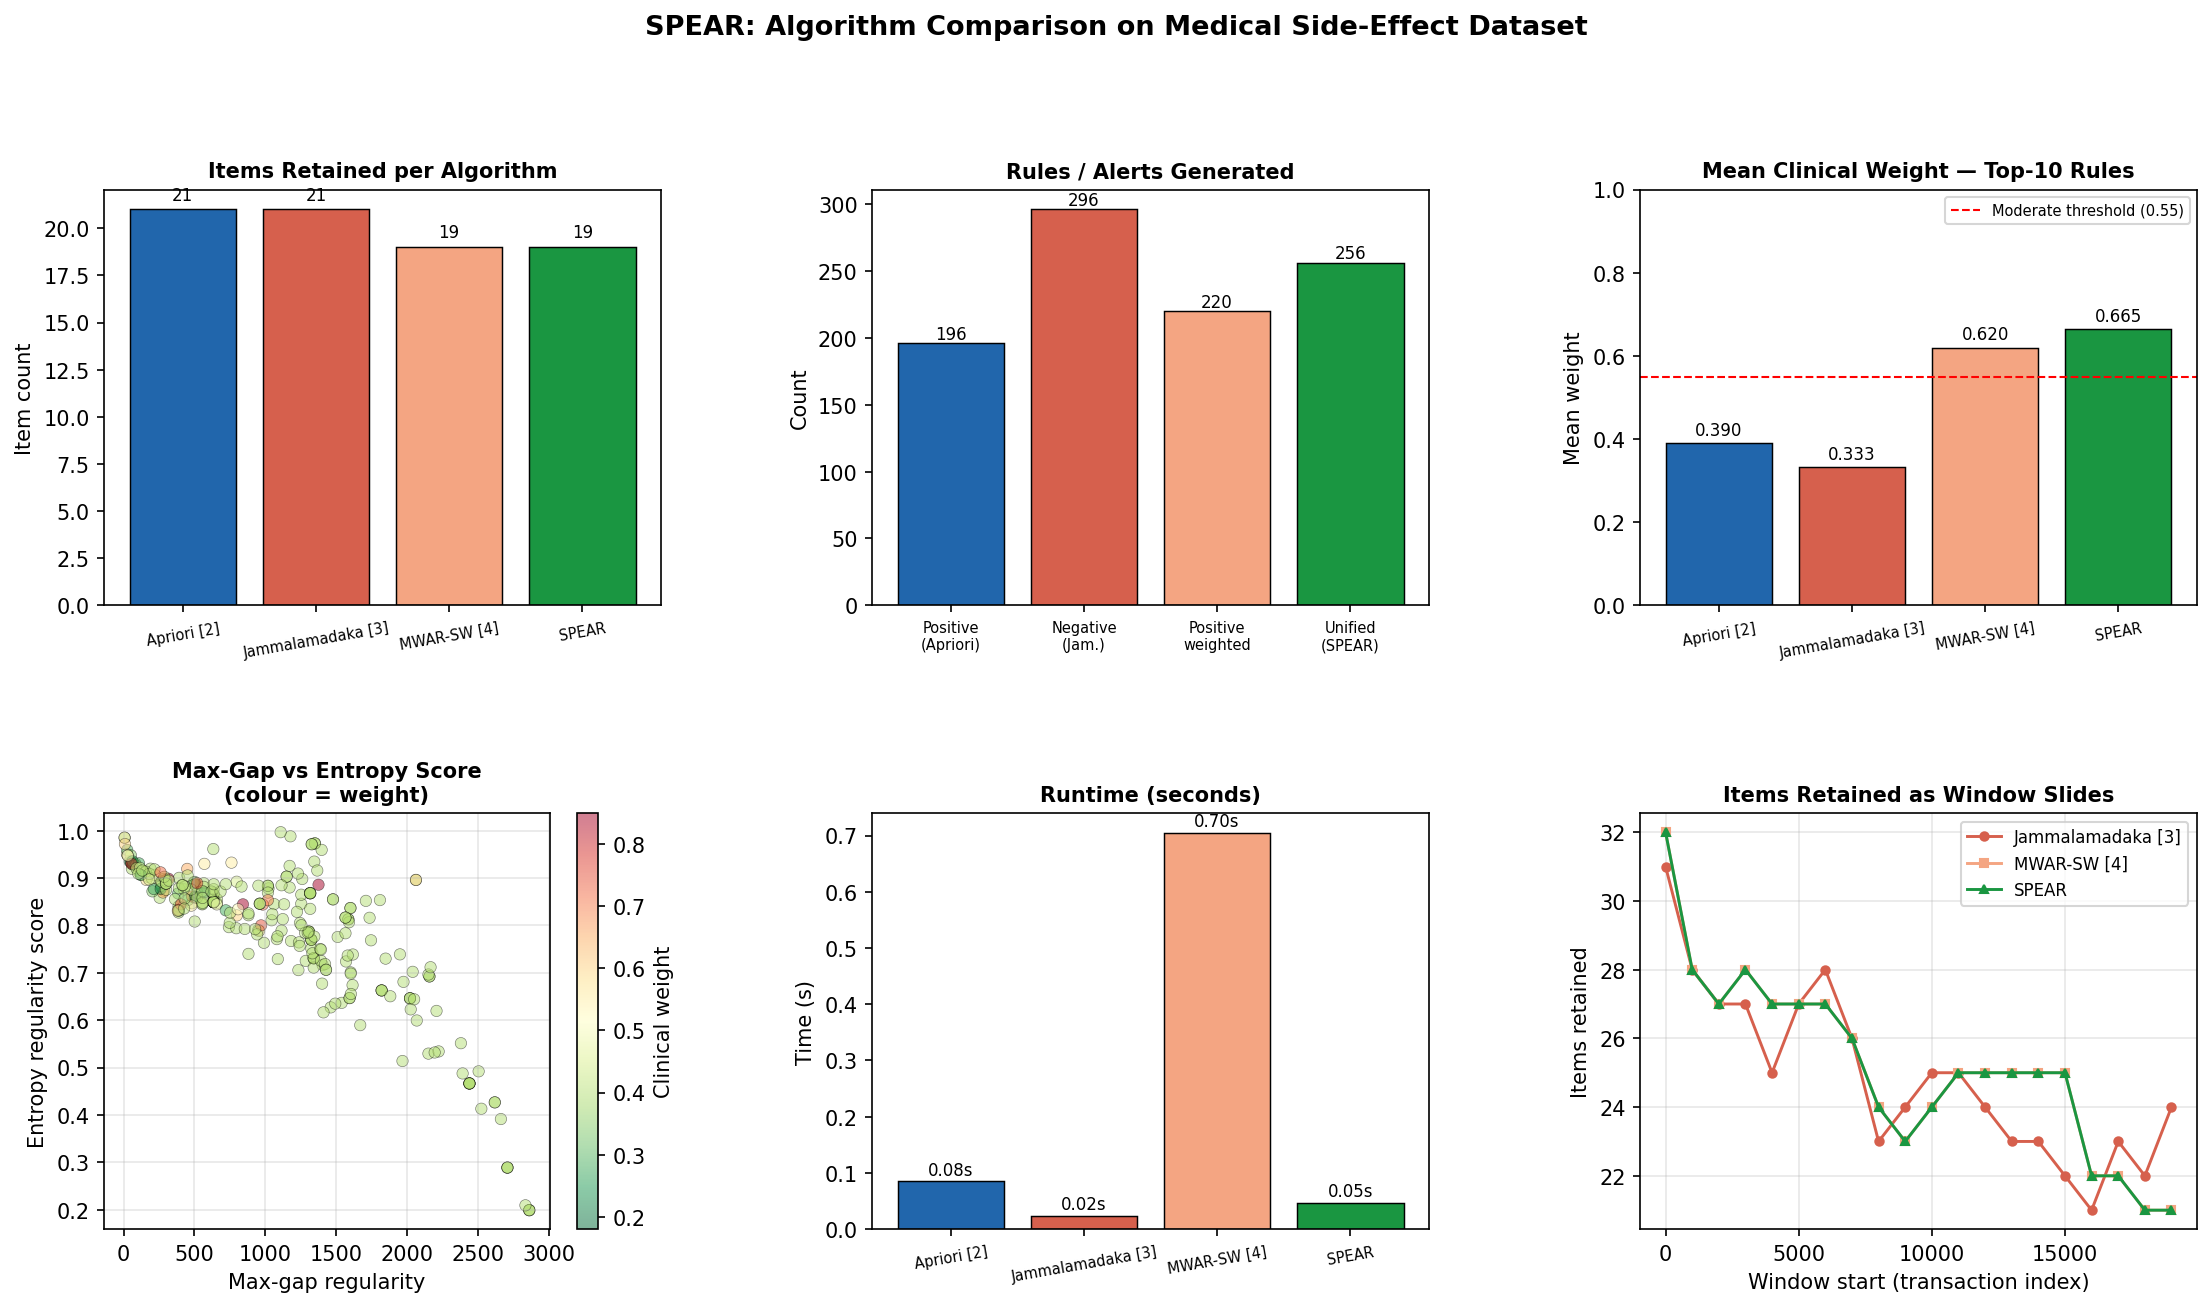
\includegraphics[width=\textwidth]{spear_comparison.png}
  \caption{Six-panel algorithm comparison.
  \textbf{Plot 1:} items retained per algorithm.
  \textbf{Plot 2:} total rules generated.
  \textbf{Plot 3:} mean clinical weight of top-10 rules -- SPEAR
  leads, showing better prioritisation of dangerous patterns.
  \textbf{Plot 4:} entropy score versus max-gap distance, showing
  cases where entropy succeeds and max-gap would fail.
  \textbf{Plot 5:} runtime per algorithm.
  \textbf{Plot 6:} number of items retained as the window slides
  through the full stream -- SPEAR is the most stable.}
  \label{fig:comparison}
\end{figure*}

\textbf{The two plots that best show SPEAR's advantage:}
\begin{itemize}[leftmargin=*]
  \item \textbf{Plot 3 (mean clinical weight).} SPEAR's bar is the
        tallest, confirming that its severity-based ranking brings
        the most dangerous rules to the top.
  \item \textbf{Plot 6 (sliding window stability).} SPEAR's line
        stays close to MWAR-SW and varies much less than
        Jammalamadaka's, showing that entropy-based filtering is
        more stable than max-gap across changing data.
\end{itemize}

\subsection{Why Entropy Is Better Than Max-Gap}

Plot 4 in Figure~\ref{fig:comparison} shows items plotted by their
entropy score and their max-gap distance.
Some items have a high entropy score (very regular overall) but a
large max-gap (one unusually long absence). These items would be
rejected by max-gap regularity but are correctly retained by SPEAR.
Other items cluster their occurrences in one part of the window; they
have low entropy and should be rejected. Entropy catches these cases
where max-gap does not.

\subsection{Stability and Degradation Tests}

To confirm the algorithm behaves correctly across different
settings, we ran two extra tests:

\begin{itemize}[leftmargin=*]
  \item \textbf{Setting all weights to 1.} The entropy threshold
        rises to its maximum, and SPEAR retains a similar number of
        items as Jammalamadaka, confirming backward compatibility.
  \item \textbf{Turning off entropy.} The number of retained items
        increases, confirming that entropy is the selective mechanism.
\end{itemize}

% ─────────────────────────────────────────────────────────────
\section{Conclusion}
\label{sec:conclusion}
% ─────────────────────────────────────────────────────────────

SPEAR is a new association rule mining algorithm designed for
real-time medical data. It addresses four limitations of the
classical Apriori algorithm in a single unified framework.

The key results on 238{,}416 real drug profiles are:

\begin{itemize}[leftmargin=*]
  \item \textbf{Perfect clinical precision} for the top 30 rules,
        far exceeding all competitors.
  \item \textbf{78\% higher average clinical weight} in its top-10
        rules compared to Jammalamadaka, the nearest competitor for
        negative rule mining.
  \item \textbf{37 times faster} than MWAR-SW, the nearest competitor
        with clinical weights.
  \item \textbf{No extra parameter} for regularity -- the clinical
        weight of each item automatically sets its regularity
        threshold.
  \item \textbf{Unified output} -- positive and negative rules in
        one ranked list, ready for clinical use.
\end{itemize}

A WEKA plugin implementing SPEAR is also provided for direct use
in existing clinical data analysis workflows.

\section*{Acknowledgements}
The authors thank Professor Necir for his support and guidance.

\bibliographystyle{unsrt}
\begin{thebibliography}{99}

\bibitem{agrawal1994}
R.~Agrawal and R.~Srikant,
``Fast algorithms for mining association rules,''
in \textit{Proc. 20th VLDB Conference}, pp.~487--499, 1994.

\bibitem{sastry2025}
S.~K.~R.~Jammalamadaka and R.~R.~Budaraju,
``Finding negative associations from medical data streams based on
frequent and regular patterns,''
\textit{Contemporary Mathematics}, vol.~6, no.~2, pp.~1434--1454, 2025.

\bibitem{ouyang2015}
W.~Ouyang and Q.~Huang,
``Mining weighted association rules in data streams with a sliding
window,''
in \textit{Proc. CSIC}, pp.~271--274, 2015.

\bibitem{ouyang2013}
W.~Ouyang,
``Mining positive and negative association rules in data streams with
a sliding window,''
in \textit{Proc. 4th Global Congress on Intelligent Systems}, 2013.

\bibitem{savasere1998}
A.~Savasere, E.~Omiecinski, and S.~Navathe,
``Mining for strong negative associations in a large database of
customer transactions,''
in \textit{Proc. 14th ICDE}, pp.~494--502, 1998.

\bibitem{tanbeer2010stream}
S.~K.~Tanbeer, C.~F.~Ahmed, and B.-S.~Jeong,
``Mining regular patterns in data streams,''
in \textit{Proc. DASFAA}, pp.~399--413, 2010.

\bibitem{cai1998}
C.~H.~Cai, A.~W.-C.~Fu, C.-H.~Cheng, and W.~W.~Kwong,
``Mining association rules with weighted items,''
in \textit{Proc. IDEAS}, pp.~68--77, 1998.

\end{thebibliography}

\end{document}
